\chapter{Identification of Events with Well-Reconstructed Decay Planes} % Main chapter title

\label{Chapter4} % For referencing the chapter elsewhere, use \ref{Chapter1} 


The first part of the work presented here is a method to identify the events with well-reconstructed decay planes by applying cuts based on the uncertainty of the impact parameter magnitude. Such cuts have become necessary in order to gain the most information possible in the $\mu\rho$ ($\mu\pi\pi$) final state. For this purpose Monte Carlo (MC) samples are going to be used to study the effects of this cut. In this dataset, the IP is known without uncertainties. Therefore, analysis on the MC-samples is going to be called generator level-study. Reconstruction level indicates the combined analysis of both MC samples and detector effects, the latter giving rise to uncertainties.\\
Mathematically, the problem consists of a 3D vector \textbf{v} (physically the spacial vector of the primary vertex PV), with a given covariance matrix $\boldsymbol{\Sigma}$ encoding the squared uncertainties $\sigma^2_i$ with respect to the PV-vector components and the correlations $\sigma_{ij}$ between them. As for the nature of the processes in the detector, the distribution of these uncertainties can be assumed to be Gaussian, its contour lines describing three-dimensional ellipsoids centred around the primary vertex. This can be easily shown by considering the contour lines of the multivariate normal distribution
\begin{equation}
	G(\boldsymbol{x};\boldsymbol{\Sigma},\boldsymbol{\mu}=\boldsymbol{v}) = \frac{1}{\sqrt{(2\pi)^3\det\boldsymbol{\Sigma}}}\exp{\left[-\frac{1}{2}(\boldsymbol{x}-\boldsymbol{v})^T \boldsymbol{\Sigma}^{-1}(\boldsymbol{x}-\boldsymbol{v}) \right]} = C = const.
\end{equation}
and rearranging all the \textbf{x}-independent terms to the right-hand side of the equation yielding
\begin{equation}
	(\boldsymbol{x}-\boldsymbol{v})^T \boldsymbol{\Sigma}^{-1}(\boldsymbol{x}-\boldsymbol{v}) = -2\cdot\ln\left(C\cdot\sqrt{(2\pi)^3\det\boldsymbol{\Sigma}}\right)=K>0.
\end{equation}
The inequality holds, since both $\boldsymbol{\Sigma}$ and $\boldsymbol{\Sigma^{-1}}$ are positive definite, defining the ellipsoid, similar to its 2D version shown in Fig. \ref{fig:ellipse}.
\begin{figure}[h]
	\centering
	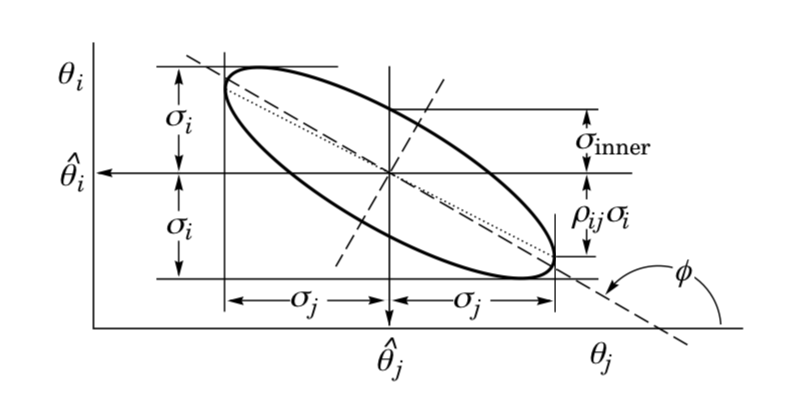
\includegraphics[width=0.7\linewidth]{Figures/ellipsoid}
	\caption{Countour lines of a 2D normal distribution \parencite{PDG_source}}
	\label{fig:ellipse}
\end{figure}\\
In the following, consider the 3-dimensional impact parameter vector \textbf{d} in the reference frame centred around \textbf{v}. Since the direction of \textbf{d} is the physically important quantity in the impact parameter method described in section \ref{sec:IP_method}, it is crucial to exclude the cases where the reconstructed IP points to a different direction then the generated IP vector, giving false results regarding the angle between the $\tau$ decay planes $\varphi^*$. During a real measurement these cases are impossible to identify, therefore one has to apply cuts on the impact parameter based on the uncertainties of \textbf{v}.\\
For this reason, consider the variable $\alpha$, defined as
\begin{equation}
	\alpha = \frac{d}{\sigma_{d}},
\end{equation}
where $d = |\boldsymbol{d}|$, the length of the IP vector. This newly defined variable contains information about the magnitude of the IP from the primary vertex expressed in units of the uncertainty $\sigma_{d}$. In the case where $\alpha = 1$, this means that the endpoints of the IP vector lies on the surface of the uncertainty ellipsoid of the PV. It can be therefore assumed that the chance of a more precisely reconstructed impact parameter direction is higher if the IP vector endpoint is further away from the uncertainty ellipsoid of the primary vertex.\\
Now it remains to determine $\sigma_{d}$. For this, first consider the length of the IP vector $d$
\begin{equation}
	d = \sqrt{d_x^2+d_y^2+d_z^2}
\end{equation}
with which $\sigma_{d}$ can be expressed through the error propagation formula \parencite{Book_error_prop}
\begin{equation}
	\sigma_{d}^2 = \mathbf{J}^T \, \boldsymbol{\Sigma} \, \mathbf{J}
\end{equation}
where \textbf{J} denotes the Jacobian defined as
\begin{equation}
	\mathbf{J} = \nabla d
\end{equation}
with the nabla operator acting on the components of \textbf{d}. This yields however
\begin{equation}
	\nabla d = \partial_i \, d \, \boldsymbol{e}_i = \frac{d_i}{d}\boldsymbol{e}_i = \frac{\boldsymbol{d}}{d} = \boldsymbol{\hat{d}},
\end{equation}
meaning the the uncertainty $\sigma_{d}$ can be written as
\begin{equation}
	\sigma_{d} = \sqrt{\boldsymbol{\hat{d}}^T \, \boldsymbol{\Sigma} \, \boldsymbol{\hat{d}}}
\end{equation}
Now it remains to demonstrate the outputs of such a cut which are summarised in Fig. \ref{fig:lambda_dist}-\ref{fig:lambdacuts_CP}. In Fig. \ref{fig:lambda_dist} the distributions of both $d$ and $\sigma_{d}$ are displayed, which then, define the distribution of the cut parameter $\alpha$ shown in Fig. \ref{fig:IP_magOverLambda_dist}. In Fig. \ref{fig:lambdacuts_angles} (for a CP even scenario in the $\mu\rho$ final state), one can immediately observe the filtering of events where the uncertainty is of the same order as the IP magnitude itself, leading to smaller differences between the generated and reconstructed data. This results in case of $\frac{d}{\sigma_d}\geq7$ in the disappearance of events, where the angle between generated and reconstructed data is greater than 2rad. Similarly promising results can be observed in Fig. \ref{fig:lambdacuts_CP} where one can immediately see the increase in amplitude of the distribution converging to more recognisable $\sin$-like shape.\\
\begin{figure}[h]
	\centering
	\subfigure{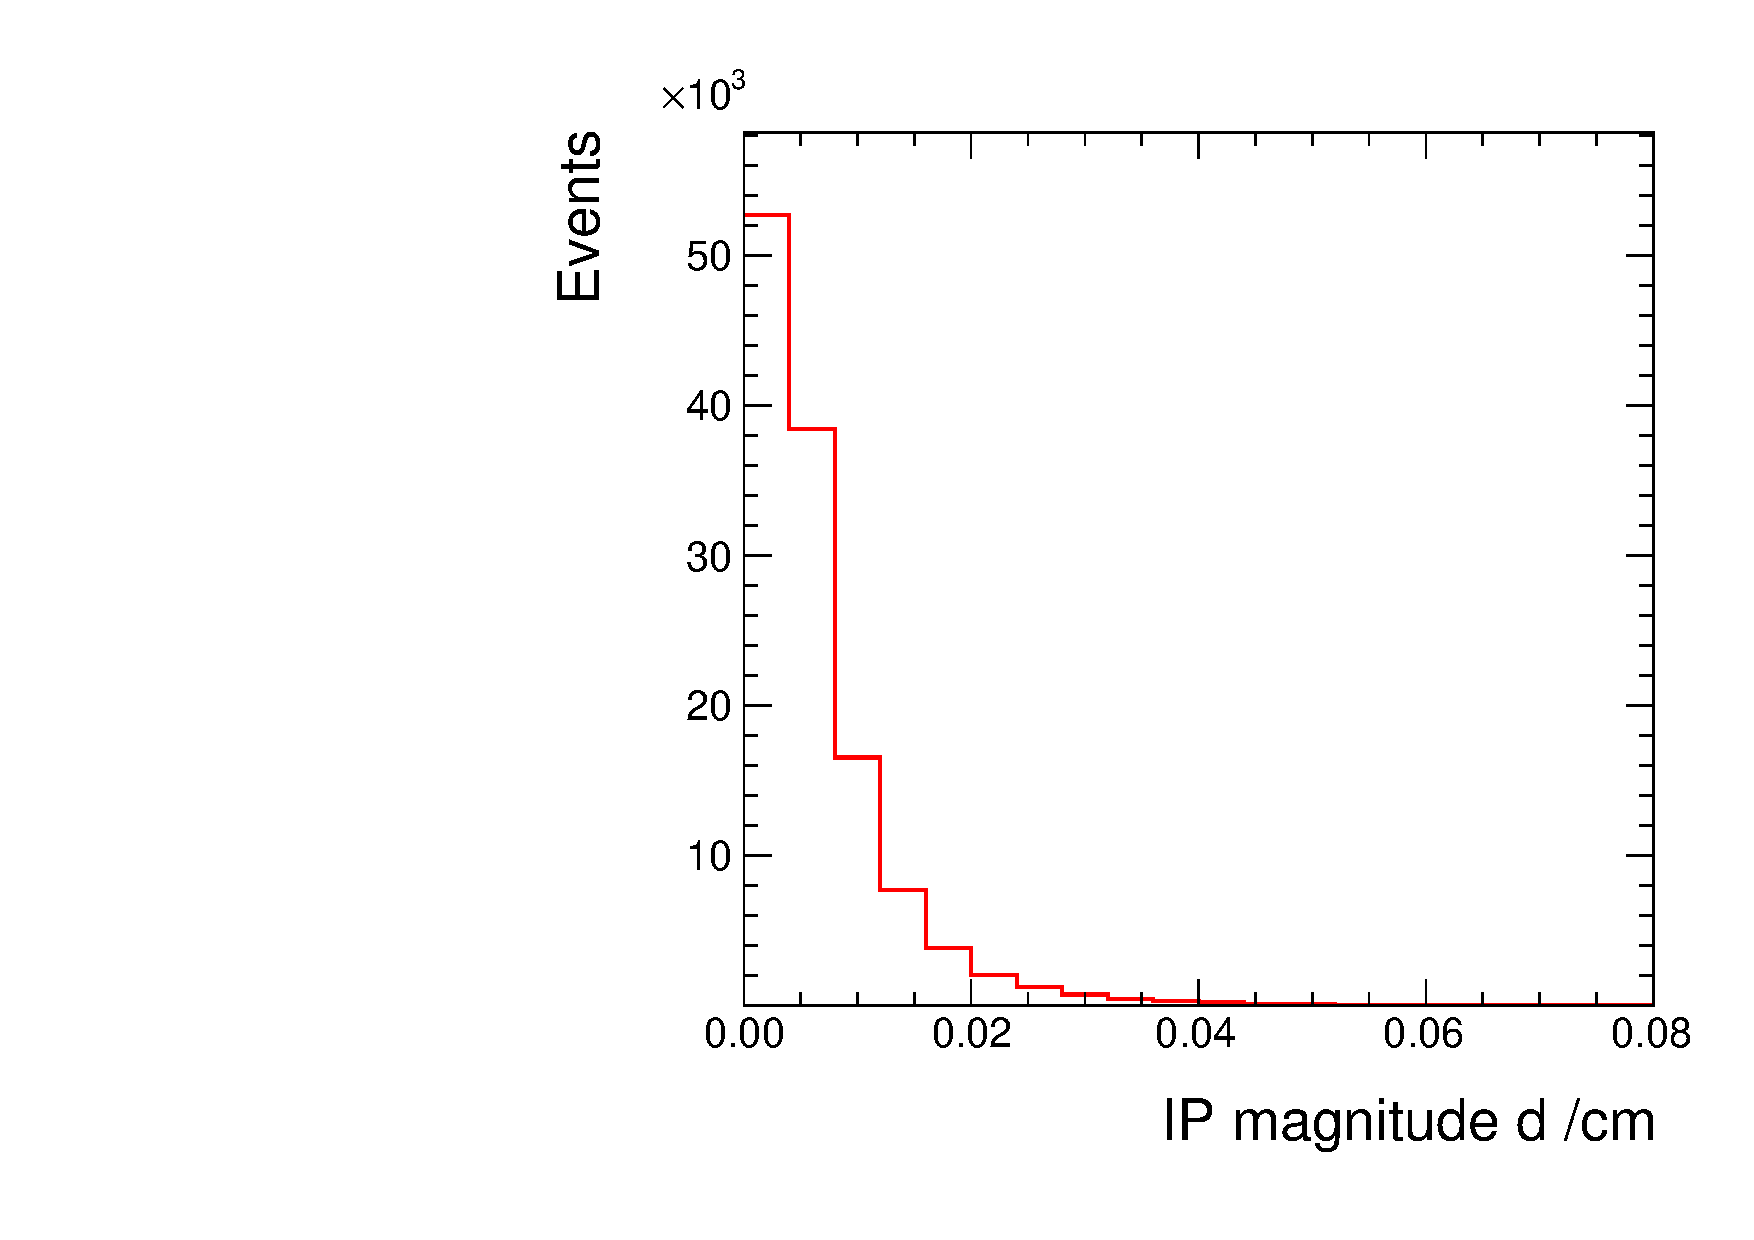
\includegraphics[width=0.4\linewidth]{Figures/IP_mag.pdf}}
	\subfigure{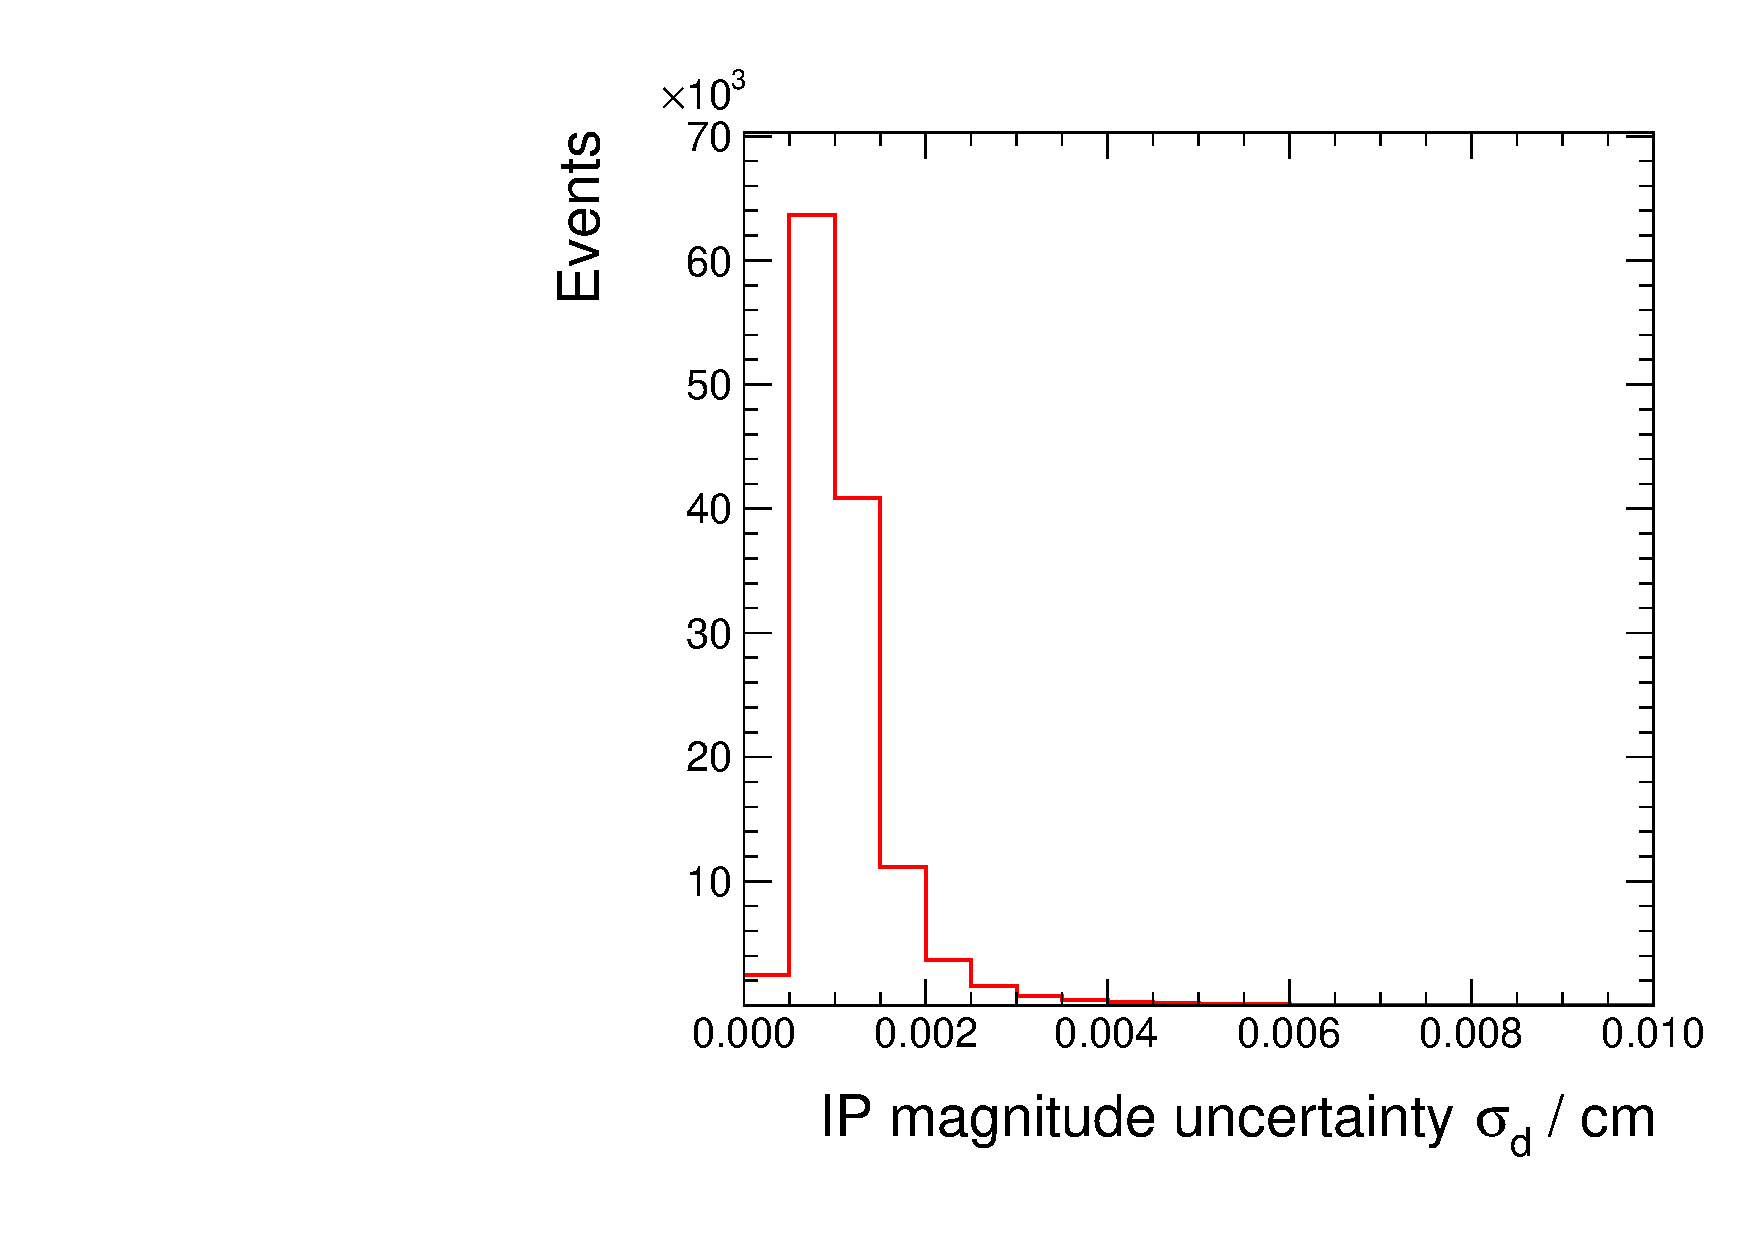
\includegraphics[width=0.4\linewidth]{Figures/IP_mag_err.pdf}}
	\caption{The distribution of IP vector magnitudes $d$ and its uncertainty $\sigma_{d}$ originating from the primary vertex in the $\mu\rho$ decay mode}
	\label{fig:lambda_dist}
\end{figure}
\begin{figure}[h]
	\centering
	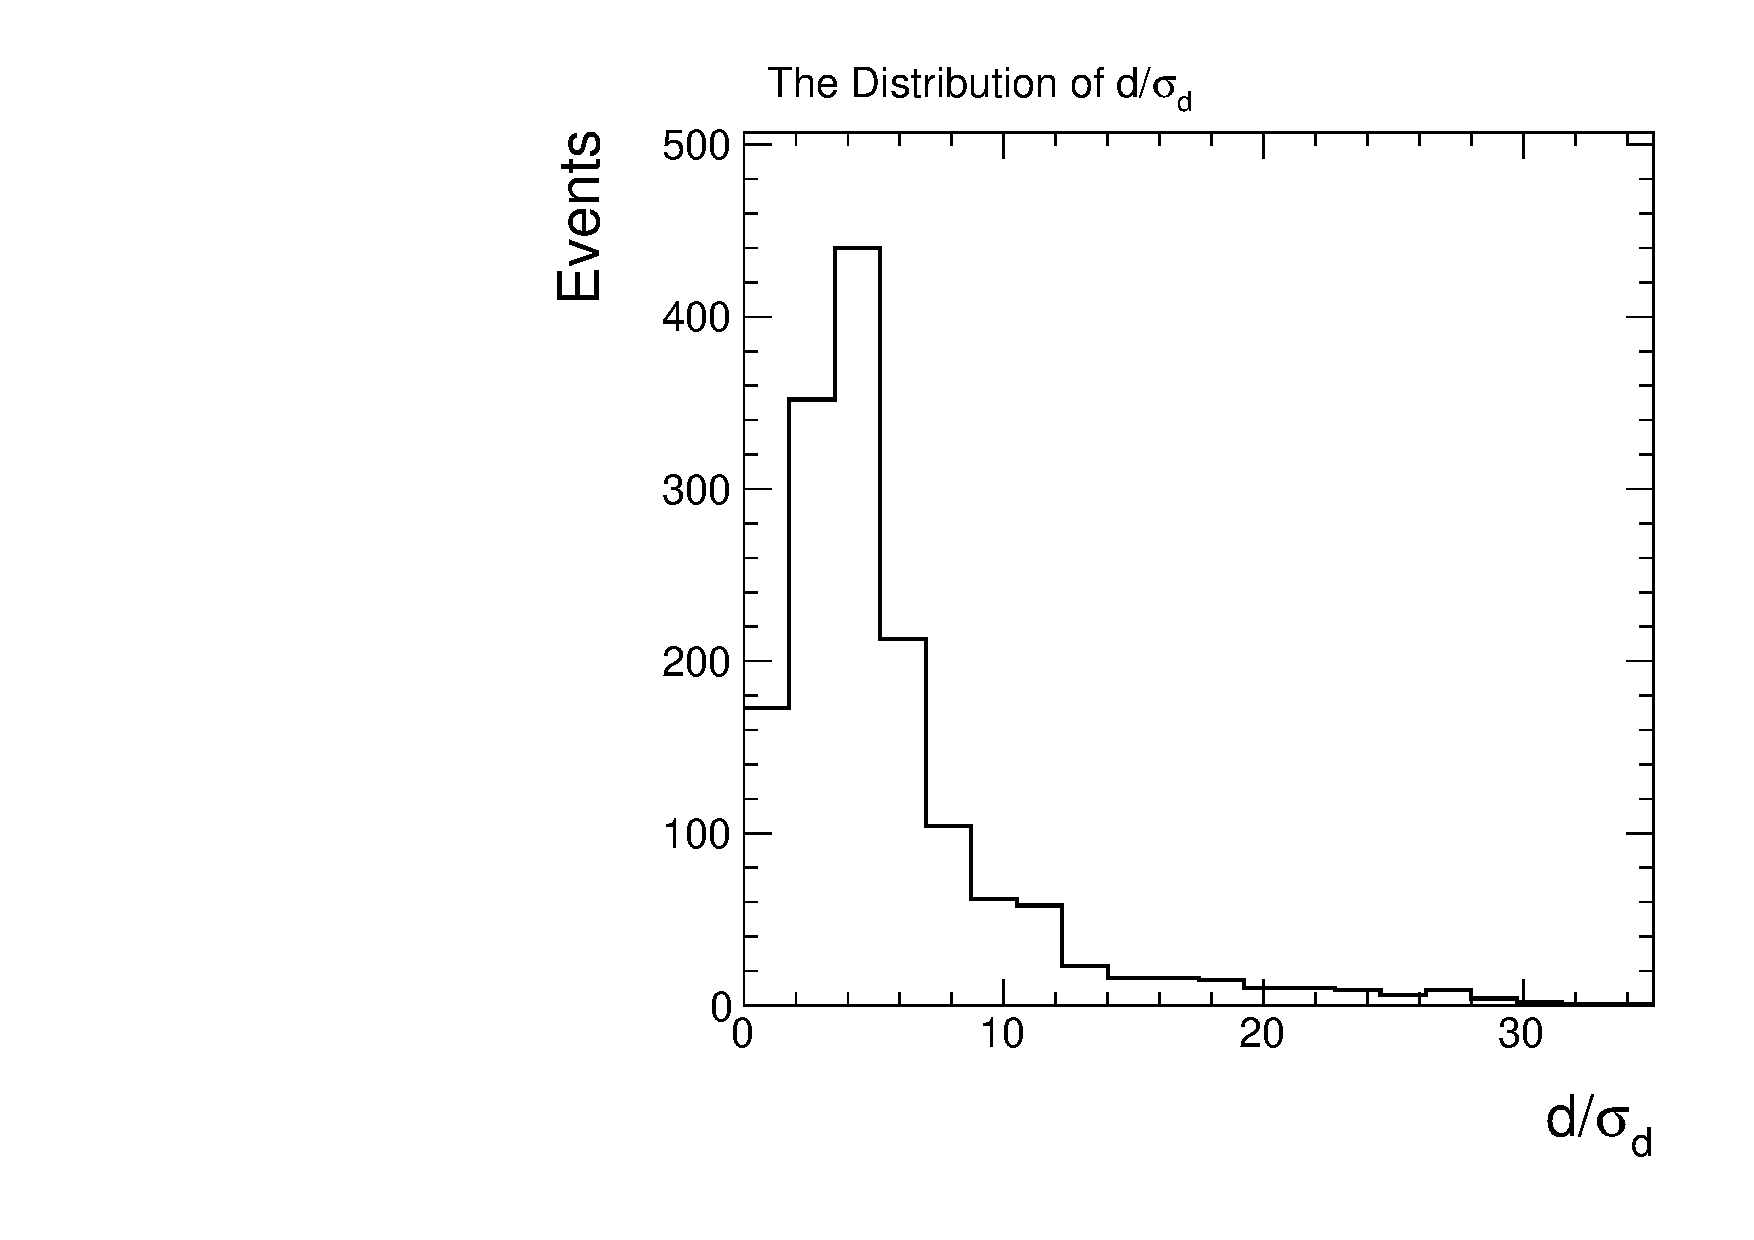
\includegraphics[width=0.6\linewidth]{Figures/IP_mag_IP_Over_err.pdf}
	\caption{The distribution of $\frac{d}{\sigma_d}$ in the $\mu \rho$ decay mode}
	\label{fig:IP_magOverLambda_dist}
\end{figure}
\begin{figure}[h]
	\centering
	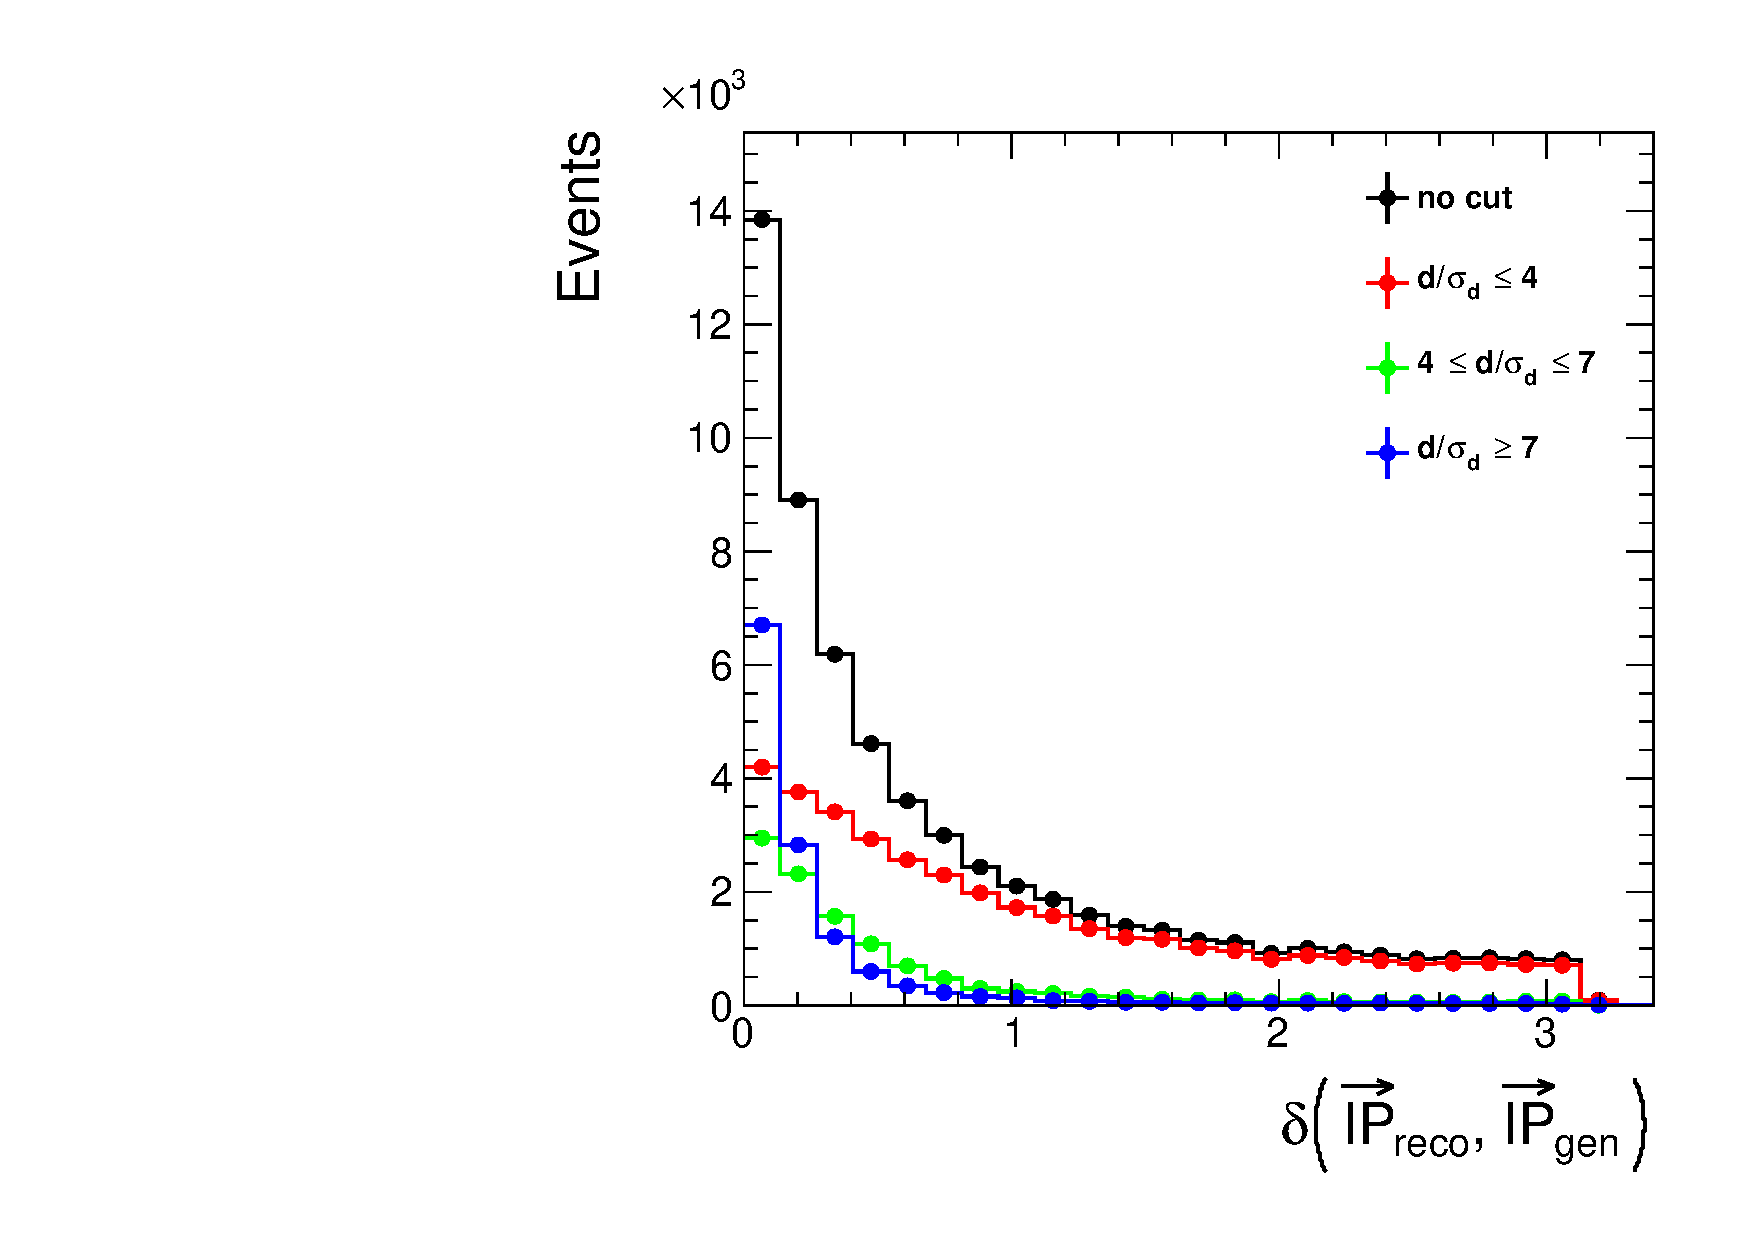
\includegraphics[width=0.7\linewidth]{Figures/deltaGenRecoIP1.pdf}
	\caption{The study of the 3D angle between the generated and reconstructed IP vectors in the $\mu\rho$ decay mode. One can observe the steady disappearance of events with small IP vectors with respect to the uncertainty ellipsoid.}
	\label{fig:lambdacuts_angles}
\end{figure}
\begin{figure}[h]
	\centering
	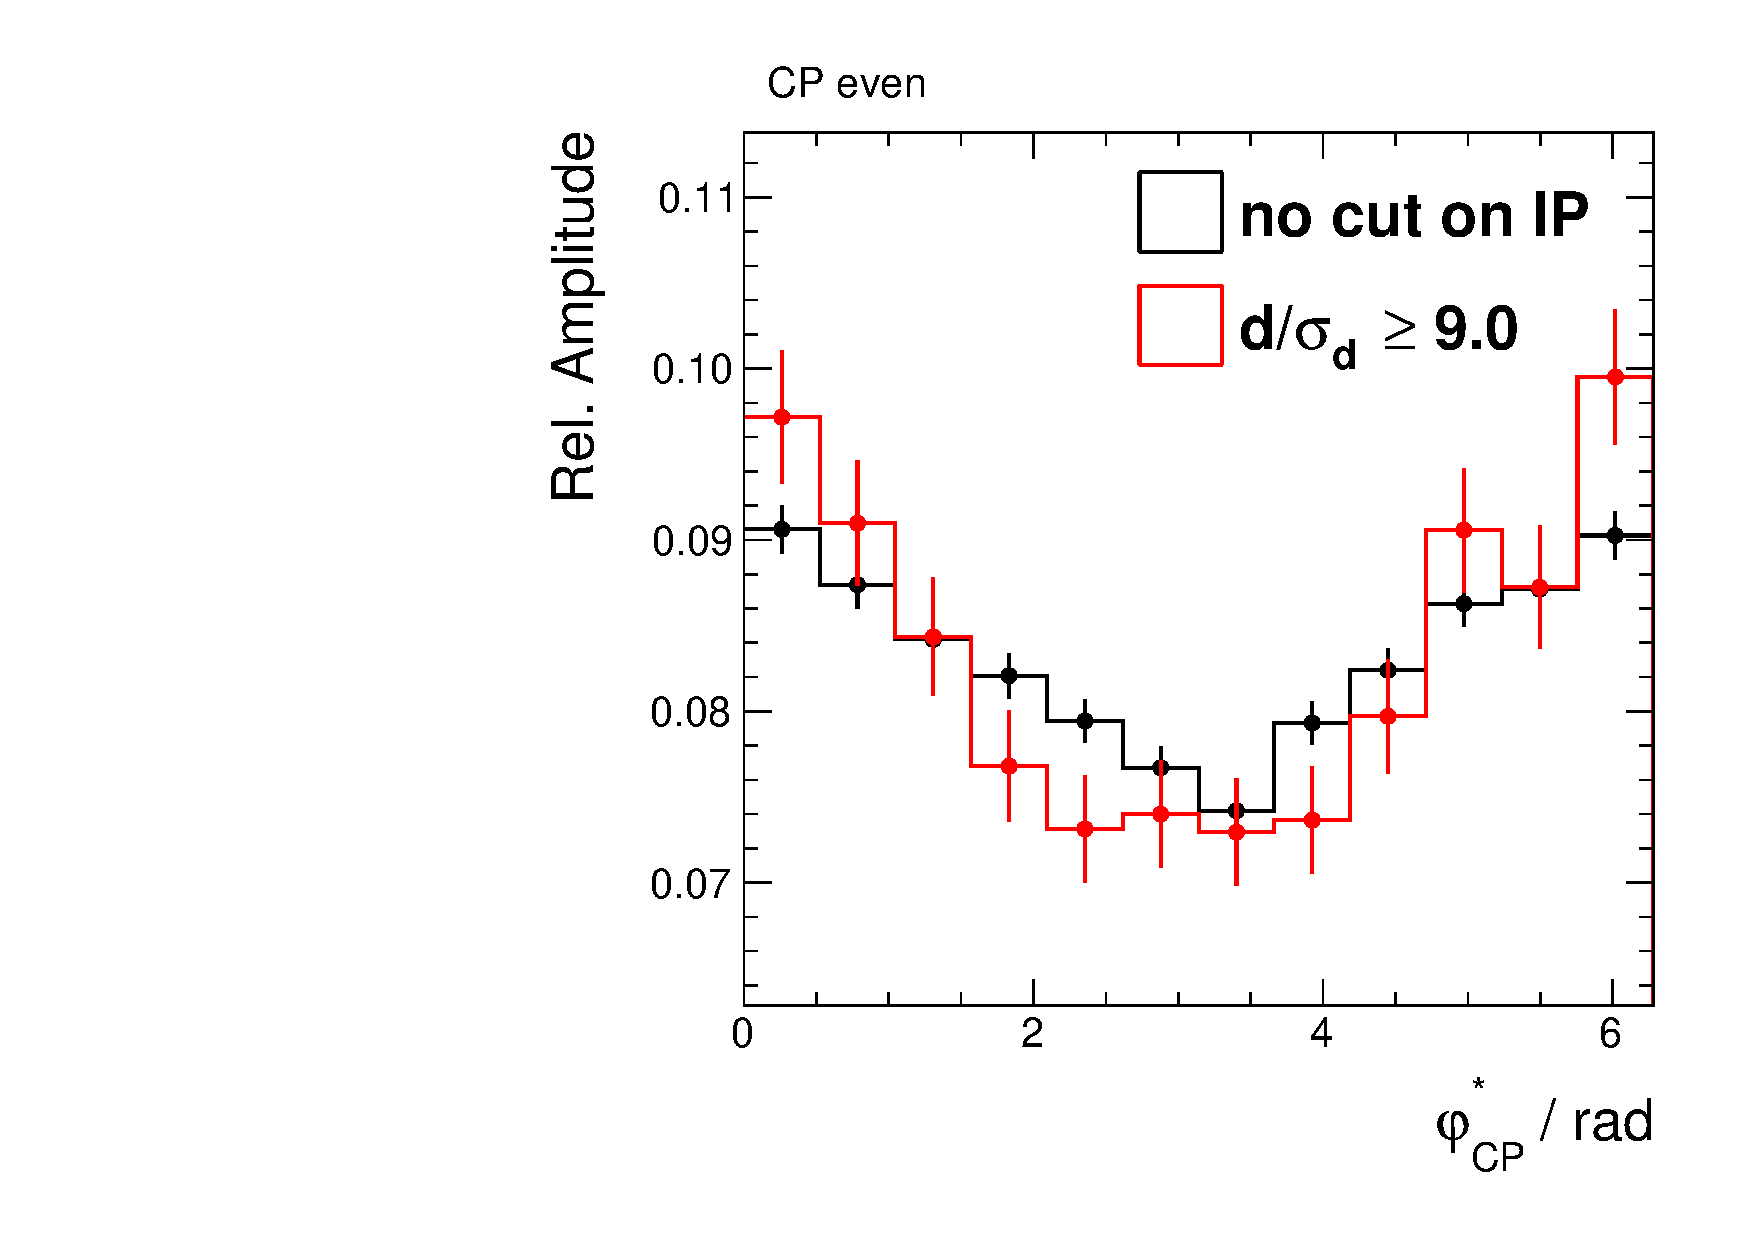
\includegraphics[width=0.7\linewidth]{Figures/recoPhiStarCPCombMerged_norefit_CPeven.pdf}
	\caption{The influence of $\alpha$-cuts on a CP-even scenario in the $\mu\rho$ decay mode. The influence of the selection of well-reconstructed decay planes can be immediately seen by the increase in the amplitude of the distribution in red.}
	\label{fig:lambdacuts_CP}
\end{figure}\\
To summarise, an efficient way of event selection has been found, which helps to reduce the influence of the primary vertex uncertainty concerning the direction of the IP vector. In order to complete the analysis, one should not neglect the uncertainty ellipsoid around the "other end" of the PV vector, which corresponds to a point on the track of the particle. Such an additional term however would only increase the total uncertainty with respect to $\sigma_{d}$ and therefore the influence of $\alpha$ on the distribution $\frac{d}{\sigma_d}$.